\section{Session 17. Hidden Markov Models}


  HMMs are probably the most popular directed graphical model out there. They are used in many sequential and temporal domains:
  \begin{itemize}
    \item speech recognition,
    \item handwriting recognition,
    \item visual target tracking and localization,
    \item machine translation,
    \item robot localization,
    \item gene prediction,
    \item time-series analysis,
    \item natural language processing and part-of-speech recognition,
    \item stochastic control,
    \item protein folding, ...
  \end{itemize}

  In HMMs, the random variables are divided into hidden states (phonemes, letters, target location) and observations (audio signal, pen strokes, target image). The goal is to predict the states from observations.

  What is this?
\begin{center}
  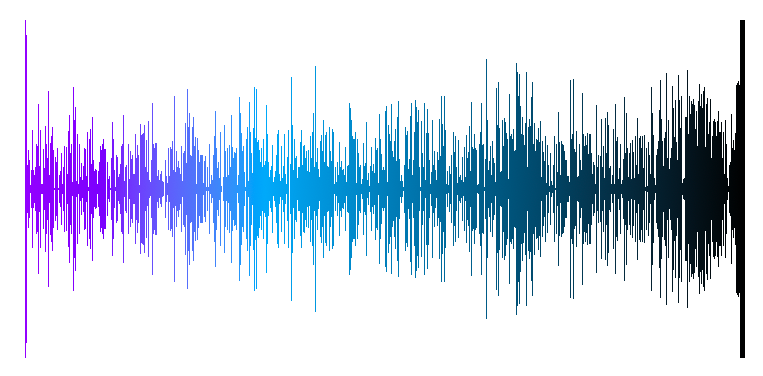
\includegraphics[width=0.7\linewidth]{../figures/SultansofSwing.png}
\end{center}

We can start wth the graphical representation of the HMM
\begin{center}
 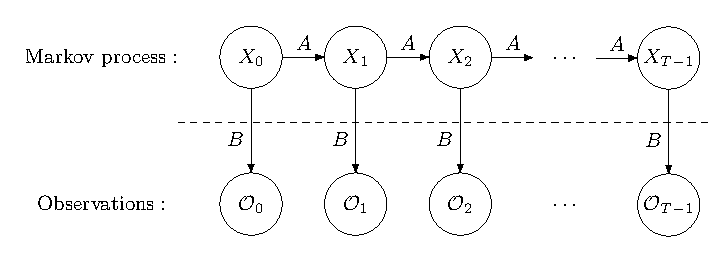
\includegraphics[width=0.7\linewidth]{../figures/HMM.pdf}
\end{center}

To learn more on HMM:
\begin{itemize}
   \item \url{https://alliance.seas.upenn.edu/~cis520/wiki/index.php?n=Lectures.HMMs#toc7}
   \item \url{http://www.columbia.edu/~mh2078/MachineLearningORFE/HMMs_MasterSlides.pdf}
\end{itemize}

\subsection{Discrete Evenet Simulations (DES)}
  \begin{center}
    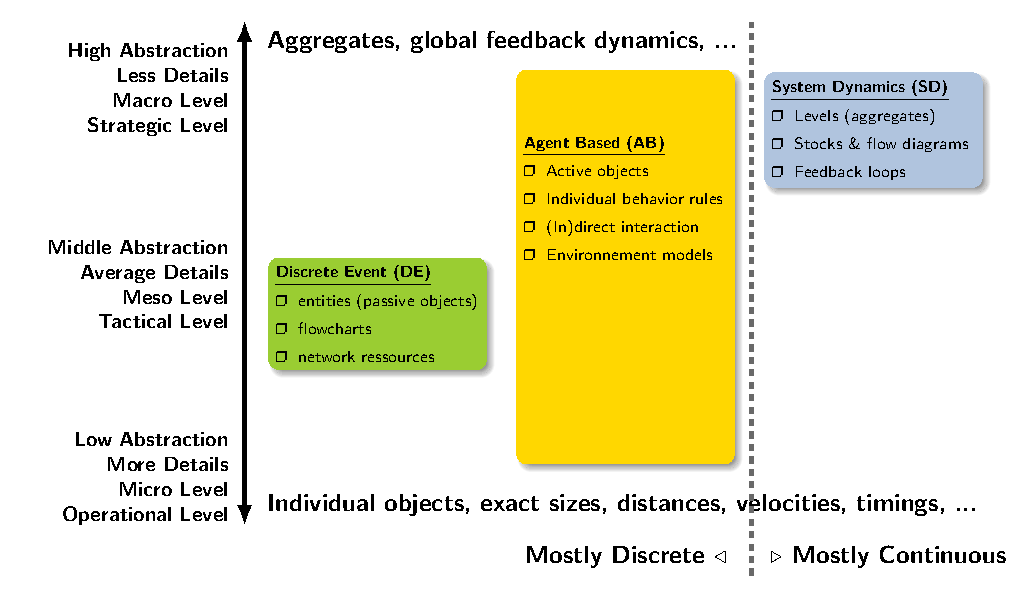
\includegraphics[width=0.7\linewidth]{../figures/simulation.pdf}
  \end{center}
  Taken from \url{https://texample.net/tikz/examples/simulation-abstraction/}
